\chapter{अवरक्त स्पेक्ट्रमिकी}\label{ch:g11:infrared}

प्रयोगशाला की एक शेल्फ़ पर रंगहीन द्रव की एक बोतल रखी है, जिसका लेबल फट चुका
है। वह कोई \omterm{def:g11:functional-groups:alcohol}{ऐल्कोहॉल}, कोई \omterm{def:g11:functional-groups:carbonyl}{कीटोन} या कोई अम्ल हो सकता है: तीन ऐसे परिवार जो बोतल में
बिल्कुल एक जैसे दिखते हैं। अवरक्त स्पेक्ट्रममापी के क्रिस्टल पर रखी एक बूँद, दो मिनट
का इंतज़ार, और स्क्रीन पर एक आलेख प्रकट होता है जो इस प्रश्न का उत्तर देता है। \omterm{def:g7:atoms-and-molecules:molecule}{अणु} के
आबंध कंपन करते हैं, और हर प्रकार का आबंध अपनी आवृत्तियों का अवरक्त प्रकाश
अवशोषित करता है: \omterm{def:g11:infrared:spectrum}{अवरक्त स्पेक्ट्रम} मौजूद आबंधों की एक सूची है।

\begin{recall}
\omterm{def:g11:functional-groups:functional-group}{क्रियात्मक समूह} और परिवार (\cref{ch:g11:functional-groups})। \omterm{def:g11:absorbance:spectrum}{अवशोषण
स्पेक्ट्रम} दिखाता है कि कोई पदार्थ हर तरंगदैर्घ्य पर कितना प्रकाश अवशोषित करता है
(\cref{ch:g11:absorbance})। \omterm{def:g11:polarity-and-cohesion:hydrogen-bond}{हाइड्रोजन आबंध} \ce{O-H}
समूहों को पड़ोसी \omterm{def:g7:atoms-and-molecules:molecule}{अणुओं} से जोड़ते हैं (\cref{ch:g11:polarity-and-cohesion})।
\end{recall}

\section{आबंध कंपन करते हैं}

\omterm{def:g10:lewis-and-shape:covalent-bond}{सहसंयोजी आबंध} दृढ़ नहीं होता: दोनों \omterm{def:g7:atoms-and-molecules:atom}{परमाणु} कंपन करते हैं, प्रति सेकंड लाखों करोड़
बार पास आते और दूर जाते हैं, एक स्प्रिंग से जुड़ी दो गेंदों की तरह। अधिक कड़ी
स्प्रिंग (एकल के बजाय \omterm{def:g10:lewis-and-shape:multiple-bond}{द्विआबंध}) या हल्की गेंदें (कार्बन \omterm{def:g7:atoms-and-molecules:atom}{परमाणु} के बजाय हाइड्रोजन
\omterm{def:g7:atoms-and-molecules:atom}{परमाणु}) अधिक तेज़ी से कंपन करती हैं। कोई आबंध ऐसा अवरक्त प्रकाश अवशोषित कर सकता है
जिसकी आवृत्ति उसके अपने कंपन से मेल खाए: आँख को अदृश्य अवरक्त प्रकाश की तरंगदैर्घ्य
कुछ माइक्रोमीटर से कुछ दसियों माइक्रोमीटर तक होती है।

\begin{omfigure}
\begin{tikzpicture}[font=\small]
  \node[aC] (c) at (0,0) {};
  \node[aO] (o) at (2.2,0) {};
  \draw[decorate, decoration={coil, aspect=0.4, segment length=4pt,
    amplitude=4pt}, thick, black!60] (c.east) -- (o.west);
  \draw[<->, omProp, thick] (-0.9,0) -- (-0.45,0);
  \draw[<->, omProp, thick] (2.65,0) -- (3.1,0);
  \node[anchor=north] at (1.1,-0.5) {खिंचता और सिकुड़ता आबंध};
  \node[aO] (o1) at (5.3,0) {};
  \node[aH] (h1) at (6.7,0) {};
  \draw[decorate, decoration={coil, aspect=0.4, segment length=3pt,
    amplitude=3pt}, thick, black!60] (o1.east) -- (h1.west);
  \draw[<->, omProp, thick] (7.0,0) -- (7.7,0);
  \node[anchor=north, align=center] at (6.2,-0.5) {हल्का हाइड्रोजन परमाणु:\\ तेज़ कंपन};
\end{tikzpicture}

{\small दो गेंदों के बीच की स्प्रिंग के रूप में चित्रित एक आबंध। उसके कंपन की
आवृत्ति आबंध की कठोरता और \omterm{def:g7:atoms-and-molecules:atom}{परमाणुओं} के द्रव्यमानों से तय होती है;
उस आवृत्ति का अवरक्त प्रकाश अवशोषित होता है।}
\end{omfigure}

\begin{definition}[तरंग संख्या]\label{def:g11:infrared:wavenumber}
किसी प्रकाश की \emph{तरंग संख्या}\index{तरंग संख्या} $\sigma$ उसकी तरंगदैर्घ्य
का व्युत्क्रम है, $\sigma = 1/\lambda$। अवरक्त स्पेक्ट्रमिकी में
इसे \si{cm^{-1}} में व्यक्त किया जाता है: एक सेंटीमीटर में तरंगदैर्घ्यों की संख्या।
बड़ी तरंग संख्या का अर्थ है छोटी तरंगदैर्घ्य और
तेज़ कंपन।
\end{definition}

\begin{example}[तरंग संख्या से तरंगदैर्घ्य तक]\label{ex:g11:infrared:convert}
$\sigma = \qty{2000}{cm^{-1}}$ पर स्थित पट्ट
$\lambda = 1/2000 = \qty{5.0e-4}{cm} = \qty{5.0}{\micro m}$ के संगत है। \omterm{def:g11:infrared:spectrum}{अवरक्त
स्पेक्ट्रम} आम तौर पर \qty{4000}{cm^{-1}} (\qty{2.5}{\micro m}) से
\qty{500}{cm^{-1}} (\qty{20}{\micro m}) तक जाते हैं।
\end{example}

\section{अवरक्त स्पेक्ट्रम पढ़ना}

\begin{definition}[अवरक्त स्पेक्ट्रम, पारगम्यता]\label{def:g11:infrared:spectrum}
किसी दी गई \omterm{def:g11:infrared:wavenumber}{तरंग संख्या} पर किसी नमूने की \emph{पारगम्यता}\index{पारगम्यता} $T$
उससे पार निकलने वाले अवरक्त प्रकाश का प्रतिशत है: कुछ भी अवशोषित न हो
तो \qty{100}{\percent}। किसी यौगिक का \emph{अवरक्त
स्पेक्ट्रम}\index{अवरक्त स्पेक्ट्रम} \omterm{def:g11:infrared:wavenumber}{तरंग संख्या} के विरुद्ध $T$ का आलेख है,
जिसे परिपाटी के अनुसार बाएँ से दाएँ घटती \omterm{def:g11:infrared:wavenumber}{तरंग संख्याओं} के साथ
बनाया जाता है।
\end{definition}

\begin{definition}[अवशोषण पट्ट, अंगुलिछाप क्षेत्र]\label{def:g11:infrared:band}
\emph{अवशोषण पट्ट}\index{अवशोषण पट्ट} \omterm{def:g11:infrared:spectrum}{पारगम्यता} में एक गिरावट है: उन \omterm{def:g11:infrared:wavenumber}{तरंग
संख्याओं} का प्रकाश किसी आबंध द्वारा अवशोषित होता है। उसकी
स्थिति बताती है कि कौन-सा आबंध है, उसकी चौड़ाई और गहराई चित्र को पूरा करती हैं।
लगभग \qty{1500}{cm^{-1}} से नीचे स्पेक्ट्रम ऐसे पट्टों से भरा होता है
जो पूरे \omterm{def:g7:atoms-and-molecules:molecule}{अणु} पर निर्भर करते हैं: यह \emph{अंगुलिछाप
क्षेत्र}\index{अंगुलिछाप क्षेत्र} किसी ज्ञात स्पेक्ट्रम से तुलना करके यौगिक को
पहचानता है, पर आबंध-दर-आबंध पढ़ना कठिन है।
\end{definition}

\begin{inthelab}[स्पेक्ट्रम रिकॉर्ड करना]
अब ज़्यादातर विद्यालयों और विश्वविद्यालयों के स्पेक्ट्रममापी हीरे का एक छोटा क्रिस्टल
इस्तेमाल करते हैं: द्रव की एक बूँद, या क्लैंप से दबाए गए ठोस के कुछ दाने, क्रिस्टल
पर रखे जाते हैं, और उसकी सतह को छूकर गुज़रने वाला अवरक्त किरणपुंज नमूने की
जाँच करता है। पहले साफ़ क्रिस्टल रिकॉर्ड किया जाता है (``पृष्ठभूमि''), जो
रिक्त विलयन की भूमिका निभाता है। दो नमूनों के बीच क्रिस्टल को टिशू और थोड़े-से
\omterm{def:g6:solutions-and-solubility:solute}{विलायक} से साफ़ किया जाता है।
\end{inthelab}

\section{अभिलाक्षणिक पट्ट}

\begin{proposition}[हर प्रकार के आबंध का अपना पट्ट होता है]\label{prop:g11:infrared:bands}
% ledger: ir:OH-free, ir:OH-bonded, ir:OH-acid, ir:NH, ir:CH, ir:CO-aldehyde, ir:CO-ketone, ir:CO-ester, ir:CO-acid, ir:CC-double, ir:CO-single
हर प्रकार का आबंध \omterm{def:g11:infrared:wavenumber}{तरंग संख्याओं} के एक अभिलाक्षणिक परास में अवशोषित करता है,
जो एक \omterm{def:g7:atoms-and-molecules:molecule}{अणु} से दूसरे \omterm{def:g7:atoms-and-molecules:molecule}{अणु} तक लगभग एक ही रहता है:
\begin{center}
\small
\begin{tabular}{lll}
\hline
आबंध & \omterm{def:g11:infrared:wavenumber}{तरंग संख्या} (\si{cm^{-1}}) & रूप \\
\hline
\ce{O-H}, \omterm{def:g11:polarity-and-cohesion:hydrogen-bond}{हाइड्रोजन आबंध} रहित (गैस, तनु) & लगभग 3600 & तीक्ष्ण \\
\ce{O-H}, हाइड्रोजन-आबंधित (द्रव \omterm{def:g11:functional-groups:alcohol}{ऐल्कोहॉल}) & 3300--3400 & चौड़ा, प्रबल \\
\omterm{def:g11:functional-groups:carboxylic-acid}{कार्बोक्सिलिक अम्ल} का \ce{O-H} & 2500--3300 & बहुत चौड़ा \\
\omterm{def:g11:functional-groups:amine}{ऐमीन} का \ce{N-H} & 3300--3500 & मध्यम (\ce{-NH2} के लिए दो पट्ट) \\
श्रृंखला का \ce{C-H} & 2850--2960 & प्रबल \\
\omterm{def:g11:functional-groups:carboxylic-acid}{एस्टर} का \ce{C=O} & लगभग 1735 & बहुत प्रबल, तीक्ष्ण \\
\omterm{def:g11:functional-groups:carbonyl}{ऐल्डिहाइड} का \ce{C=O} & लगभग 1730 & बहुत प्रबल, तीक्ष्ण \\
\omterm{def:g11:functional-groups:carbonyl}{कीटोन} का \ce{C=O} & लगभग 1715 & बहुत प्रबल, तीक्ष्ण \\
\omterm{def:g11:functional-groups:carboxylic-acid}{कार्बोक्सिलिक अम्ल} का \ce{C=O} & लगभग 1710 & बहुत प्रबल, अधिक चौड़ा \\
\ce{C=C} & लगभग 1650 & मध्यम \\
\omterm{def:g11:functional-groups:alcohol}{ऐल्कोहॉल} का \ce{C-O} & लगभग 1050 & प्रबल \\
\hline
\end{tabular}
\end{center}
\end{proposition}

\begin{proof}
ये परास बहुत-से यौगिकों पर मापे गए हैं। वे आबंध के अनुसार
समूहित होते हैं क्योंकि किसी आबंध का कंपन मुख्यतः स्वयं आबंध
और उसके दो \omterm{def:g7:atoms-and-molecules:atom}{परमाणुओं} पर निर्भर करता है, \omterm{def:g7:atoms-and-molecules:molecule}{अणु} के बाकी भाग पर कम।
\end{proof}

\begin{omfigure}
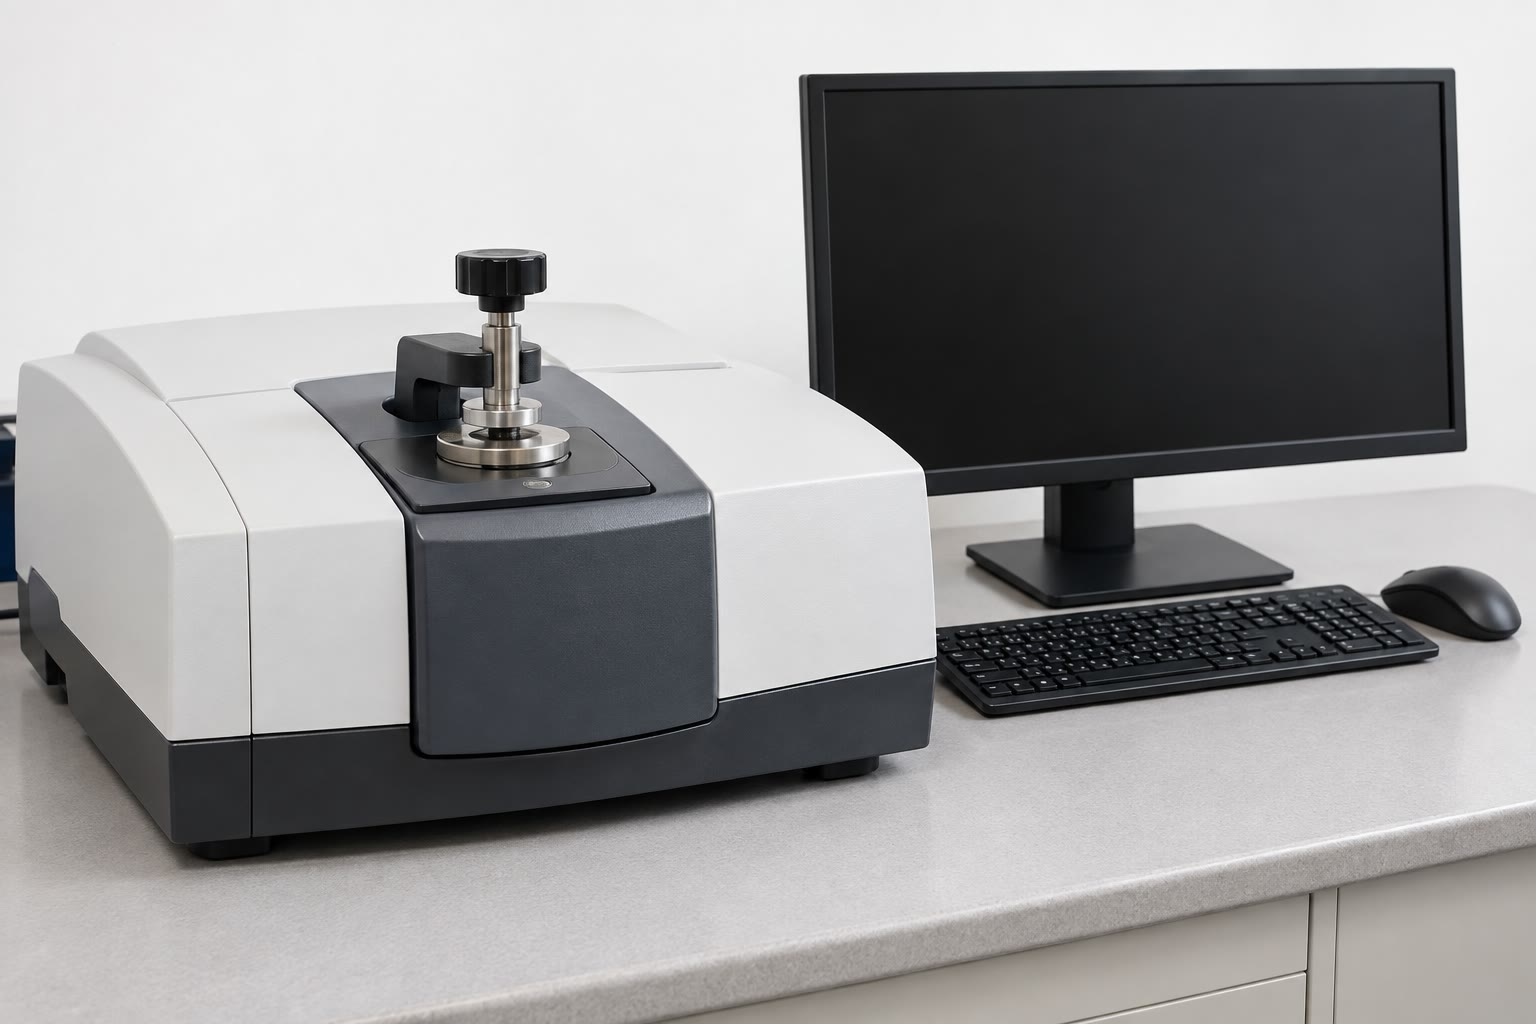
\includegraphics[width=0.48\linewidth]{images/book1/ai/g11-ftir.jpg}

{\small अपने क्रिस्टल और क्लैंप के साथ एक मेज़ पर रखा जाने वाला अवरक्त स्पेक्ट्रममापी।}
\end{omfigure}

\begin{omfigure}
\begin{tikzpicture}[font=\small, x=0.0036cm, y=0.5cm]
  % wavenumber axis reversed: x = 4000 - sigma
  \fill[black!8] (2500,0.2) rectangle (3500,7.6);
  \node[font=\footnotesize, align=center, black!60] at (3000,6.8) {अंगुलिछाप\\ क्षेत्र};
  \draw[->] (0,0) -- (3600,0) node[right] {$\sigma$};
  \foreach \s in {4000,3500,3000,2500,2000,1500,1000,500}
    \draw ({4000-\s},0) -- ({4000-\s},-0.15) node[below, font=\footnotesize] {\s};
  \node[below=12pt] at (1800,-0.3) {तरंग संख्या (\si{cm^{-1}})};
  \foreach \a/\b/\y/\c/\l in {
      3600/3600/7/omDef/{\ce{O-H} मुक्त},
      3300/3400/6/omDef/{\ce{O-H} आबंधित},
      2500/3300/5/omThm/{\ce{O-H} अम्ल},
      3300/3500/4/omMeth/{\ce{N-H}},
      2850/2960/3/black!60/{\ce{C-H}},
      1700/1740/2/omProp/{\ce{C=O}},
      1050/1050/1/black!45/{\ce{C-O}}} {
    \fill[\c, rounded corners=1pt] ({4000-\b-12},{\y-0.25}) rectangle ({4000-\a+12},{\y+0.25});
    \node[anchor=west, font=\footnotesize] at ({4000-\a+40},\y) {\l};
  }
\end{tikzpicture}

{\small मुख्य आबंध कहाँ अवशोषित करते हैं। \ce{O-H} और \ce{N-H} पट्ट
बाईं ओर हैं, \ce{C=O} पट्ट, जो आम तौर पर सबसे प्रबल होता है,
लगभग \qty{1700}{cm^{-1}} पर; \qty{1500}{cm^{-1}} से नीचे \omterm{def:g11:infrared:band}{अंगुलिछाप
क्षेत्र} है।}
\end{omfigure}

\begin{proposition}[हाइड्रोजन आबंध O--H पट्ट को चौड़ा करते हैं]\label{prop:g11:infrared:hbond}
% ledger: ir:OH-free, ir:OH-bonded, ir:ethanol-OH
जब \ce{O-H} समूह \omterm{def:g11:polarity-and-cohesion:hydrogen-bond}{हाइड्रोजन आबंधों} से जुड़े होते हैं, जैसे किसी द्रव
\omterm{def:g11:functional-groups:alcohol}{ऐल्कोहॉल} में, तो उनका पट्ट चौड़ा होता है और कम \omterm{def:g11:infrared:wavenumber}{तरंग संख्याओं} पर (लगभग
3300--\qty{3400}{cm^{-1}}) होता है; \omterm{def:g11:polarity-and-cohesion:hydrogen-bond}{हाइड्रोजन आबंधों} के बिना, जैसे गैस में, वह
तीक्ष्ण होता है और लगभग \qty{3600}{cm^{-1}} पर।
\end{proposition}

\begin{proof}
स्वीकृत: \omterm{def:g11:polarity-and-cohesion:hydrogen-bond}{हाइड्रोजन आबंध} हाइड्रोजन \omterm{def:g7:atoms-and-molecules:atom}{परमाणु} को खींचता है और
\ce{O-H} आबंध को ढीला कर देता है, जो धीमे कंपन करता है; और चूँकि हर \omterm{def:g7:atoms-and-molecules:molecule}{अणु}
थोड़ा अलग ढंग से आबंधित होता है, पट्ट एक परास में फैल जाता है।
\end{proof}

\section{क्रियात्मक समूहों की पहचान}


\begin{method}[अवरक्त स्पेक्ट्रम पढ़ना]\label{met:g11:infrared:reading}
\begin{enumerate}
  \item पहले \qty{1500}{cm^{-1}} से ऊपर देखिए; \omterm{def:g11:infrared:band}{अंगुलिछाप क्षेत्र} को
        ज्ञात स्पेक्ट्रमों से तुलना के लिए छोड़ दीजिए।
  \item लगभग \qty{1700}{cm^{-1}} पर: बहुत प्रबल पट्ट का अर्थ है \ce{C=O}
        समूह (\omterm{def:g11:functional-groups:carbonyl}{ऐल्डिहाइड}, \omterm{def:g11:functional-groups:carbonyl}{कीटोन}, अम्ल, \omterm{def:g11:functional-groups:carboxylic-acid}{एस्टर}, \omterm{def:g11:functional-groups:amine}{ऐमाइड})।
  \item 2500 और \qty{3700}{cm^{-1}} के बीच: लगभग
        \qty{3350}{cm^{-1}} पर चौड़ा पट्ट \omterm{def:g11:functional-groups:alcohol}{ऐल्कोहॉल} का \ce{O-H} है;
        2500 से \qty{3300}{cm^{-1}} तक बहुत चौड़ा पट्ट, साथ में \ce{C=O}, का अर्थ है
        \omterm{def:g11:functional-groups:carboxylic-acid}{कार्बोक्सिलिक अम्ल}; 3300--\qty{3500}{cm^{-1}} पर मध्यम पट्टों का अर्थ है
        \ce{N-H}।
  \item परिवार चुनने के लिए \omterm{def:g11:organic-skeletons:formulas}{आण्विक सूत्र} को भी साथ लीजिए, फिर अगर
        \ce{C=O} पट्ट हो तो उसकी स्थिति से पुष्टि कीजिए।
\end{enumerate}
\end{method}

\begin{omfigure}
\newcommand{\irpanel}[2]{%
\begin{tikzpicture}
\begin{axis}[width=0.96\linewidth, height=3.9cm, x dir=reverse, xmin=500,
    xmax=4000, ymin=0, ymax=105, xtick={4000,3000,2000,1000},
    /pgf/number format/1000 sep={},
    ytick={0,50,100}, tick label style={font=\scriptsize},
    label style={font=\scriptsize}, ylabel={$T$ (\%)}, axis lines*=left,
    title={\small #2}, title style={yshift=-4pt}]
  \addplot[thick, omDef] table[x=sigma, y=#1] {figdata/out/grade-11-infrared.dat};
\end{axis}
\end{tikzpicture}}
\begin{minipage}{0.49\linewidth}\irpanel{ethanolL}{A: एथेनॉल (द्रव)}\end{minipage}\hfill
\begin{minipage}{0.49\linewidth}\irpanel{ethanolG}{B: एथेनॉल (गैस)}\end{minipage}

\begin{minipage}{0.49\linewidth}\irpanel{propanone}{C: प्रोपेनोन}\end{minipage}\hfill
\begin{minipage}{0.49\linewidth}\irpanel{acid}{D: एथेनोइक अम्ल}\end{minipage}

\begin{minipage}{0.49\linewidth}\irpanel{ester}{E: एथिल एथेनोएट}\end{minipage}\hfill
\begin{minipage}{0.49\linewidth}\irpanel{amine}{F: एथेनेमीन}\end{minipage}

{\small छह यौगिकों के \omterm{def:g11:infrared:spectrum}{अवरक्त स्पेक्ट्रम}, \omterm{def:g11:infrared:wavenumber}{तरंग संख्या} \si{cm^{-1}} में
(दाईं ओर घटती हुई)। केवल अध्याय में चर्चा किए गए पट्ट
बनाए गए हैं; उनकी स्थितियाँ मापे गए स्पेक्ट्रमों और सारणियों से ली गई हैं, उनकी
आकृतियाँ एक सरल मॉडल से।}
\end{omfigure}

\begin{example}[छहों स्पेक्ट्रम पढ़ना]\label{ex:g11:infrared:six}
% ledger: ir:OH-bonded, ir:ethanol-OH, ir:CO-ketone, ir:OH-acid, ir:CO-acid, ir:CO-ester, ir:ethylethanoate-COC, ir:NH
एथेनॉल (A) लगभग \qty{3350}{cm^{-1}} पर एक चौड़ा \ce{O-H} पट्ट,
\qty{3000}{cm^{-1}} से ठीक नीचे \ce{C-H} पट्ट और लगभग \qty{1050}{cm^{-1}} पर एक
प्रबल \ce{C-O} पट्ट दिखाता है, पर लगभग \qty{1700}{cm^{-1}} पर कुछ नहीं।
गैस (B) में उसका \ce{O-H} पट्ट \qty{3666}{cm^{-1}} पर एक तीक्ष्ण रेखा
बन जाता है। प्रोपेनोन (C) में कोई \ce{O-H} पट्ट नहीं है, पर \qty{1715}{cm^{-1}} पर
एक बहुत प्रबल \ce{C=O} है। एथेनोइक अम्ल (D) दोनों दिखाता है: 2500 से
\qty{3300}{cm^{-1}} तक एक विशाल \ce{O-H} पट्ट और \qty{1710}{cm^{-1}} पर एक \ce{C=O}।
एथिल एथेनोएट (E) का \ce{C=O} \qty{1735}{cm^{-1}} पर है और एक प्रबल \ce{C-O}
लगभग \qty{1240}{cm^{-1}} पर, और कोई \ce{O-H} नहीं। एथेनेमीन (F)
\qty{3300}{cm^{-1}} से ऊपर दो मध्यम \ce{N-H} पट्ट दिखाता है।
\end{example}

\section{अभ्यास}

\begin{exercise}[$\star$]\label{exo:g11:infrared:1}
माइक्रोमीटर में तरंगदैर्घ्य में बदलिए: $\sigma = \qty{3300}{cm^{-1}}$
और $\sigma = \qty{1050}{cm^{-1}}$। कौन-सी तेज़ कंपन के
संगत है?
\end{exercise}

\begin{exercise}[$\star$]\label{exo:g11:infrared:2}
\qty{10}{\micro m} की तरंगदैर्घ्य अवशोषित होती है। \omterm{def:g11:infrared:wavenumber}{तरंग संख्या}
\si{cm^{-1}} में बताइए।
\end{exercise}

\begin{exercise}[$\star$]\label{exo:g11:infrared:3}
कौन-सा आबंध अवशोषित करता है: लगभग \qty{1715}{cm^{-1}} पर; लगभग \qty{3350}{cm^{-1}}
पर (चौड़ा); 2850 और \qty{2960}{cm^{-1}} के बीच?
\end{exercise}

\begin{exercise}[$\star$]\label{exo:g11:infrared:4}
स्पेक्ट्रम C (प्रोपेनोन) पर सबसे प्रबल पट्ट खोजिए। वह किस आबंध
का है?
\end{exercise}

\begin{exercise}[$\star$]\label{exo:g11:infrared:5}
\omterm{def:g11:infrared:spectrum}{अवरक्त स्पेक्ट्रम} \omterm{def:g11:infrared:spectrum}{पारगम्यता} अक्ष के साथ, नीचे की ओर इशारा करते पट्टों के साथ, क्यों
बनाया जाता है? $T = \qty{100}{\percent}$ का क्या अर्थ है?
\end{exercise}

\begin{exercise}[$\star\star$]\label{exo:g11:infrared:6}
एक यौगिक \ce{C4H8O} \qty{1715}{cm^{-1}} पर एक बहुत प्रबल पट्ट
दिखाता है और \qty{3000}{cm^{-1}} से ऊपर कोई पट्ट नहीं। एक दूसरा,
\ce{C4H10O}, लगभग \qty{3350}{cm^{-1}} पर एक चौड़ा पट्ट दिखाता है और लगभग
\qty{1700}{cm^{-1}} पर कोई नहीं। वे किन परिवारों के हैं? हर एक के लिए एक नाम
सुझाइए।
\end{exercise}

\begin{exercise}[$\star\star$]\label{exo:g11:infrared:7}
समझाइए कि एथेनोइक अम्ल का \ce{O-H} पट्ट इतना चौड़ा क्यों है, द्रव एथेनॉल
के पट्ट से भी अधिक चौड़ा।
\end{exercise}

\begin{exercise}[$\star\star$]\label{exo:g11:infrared:8}
एथेनॉल के स्पेक्ट्रम A और B की तुलना कीजिए। क्या बदलता है, और क्यों?
\end{exercise}

\begin{exercise}[$\star\star$]\label{exo:g11:infrared:9}
प्रोपेनैल और प्रोपेनोन दोनों \ce{C3H6O} हैं। दोनों एक प्रबल \ce{C=O}
पट्ट दिखाते हैं। क्या केवल उस पट्ट से अवरक्त उन्हें अलग पहचान सकता है? और क्या
मदद कर सकता है?
\end{exercise}

\begin{exercise}[$\star\star$]\label{exo:g11:infrared:10}
एक यौगिक \qty{1735}{cm^{-1}} पर एक प्रबल पट्ट, लगभग \qty{1240}{cm^{-1}} पर
एक प्रबल पट्ट और \qty{3000}{cm^{-1}} से ऊपर कुछ नहीं दिखाता। उसका सूत्र
\ce{C4H8O2} है। कौन-सा परिवार? क्या एथेनोइक अम्ल एक संभावना है? ब्यूटेनोइक
अम्ल?
\end{exercise}

\begin{exercise}[$\star\star$]\label{exo:g11:infrared:11}
प्रोपेन-1-ऑल का \omterm{def:g7:atoms-and-molecules:molecule}{अणु} छह स्पेक्ट्रमों में से किससे सबसे अधिक मिलता-जुलता होगा?
प्रोपेनोइक अम्ल का? समझाइए।
\end{exercise}

\begin{exercise}[$\star\star\star$]\label{exo:g11:infrared:12}
प्रोपेन-2-ऑल का ऑक्सीकरण करके प्रोपेनोन बनाया जा सकता है। एक छात्रा हर दस मिनट पर
लिए गए नमूनों के स्पेक्ट्रम रिकॉर्ड करके अभिक्रिया पर नज़र रखती है।
वर्णन कीजिए कि स्पेक्ट्रम कैसे बदलते हैं। उसे कैसे पता चलता है कि अभिक्रिया
पूरी हो गई है?
\end{exercise}

\begin{exercise}[$\star\star\star$]\label{exo:g11:infrared:13}
ब्यूटेनोइक अम्ल और एथिल एथेनोएट \omterm{def:g11:organic-skeletons:isomer}{समावयवी} हैं, \ce{C4H8O2}। उनके \omterm{def:g11:infrared:spectrum}{अवरक्त स्पेक्ट्रमों}
के बीच दो अंतरों का वर्णन कीजिए, और उन्हें समझाइए।
\end{exercise}

\begin{exercise}[$\star\star\star$]\label{exo:g11:infrared:14}
एथिल एथेनोएट का एक नमूना अपेक्षित पट्टों के अलावा लगभग \qty{3350}{cm^{-1}} पर
एक कमज़ोर चौड़ा पट्ट दिखाता है। दो अशुद्धियाँ सुझाइए जो इसका कारण हो सकती हैं
(सोचिए कि \omterm{def:g11:functional-groups:carboxylic-acid}{एस्टर} कैसे बनते हैं, और \omterm{def:g4:air-a-mixture-of-gases:air}{वायु} के बारे में)। नमूने की जाँच कैसे
की जा सकती है?
\end{exercise}

\begin{exercise}[$\star\star\star$]\label{exo:g11:infrared:15}
\omterm{def:g11:functional-groups:carbonyl}{कीटोनों} का \ce{C=O} पट्ट लगभग \qty{1715}{cm^{-1}} पर होता है, किसी
\ce{C=C} का लगभग \qty{1650}{cm^{-1}} पर, और \ce{C-O} पट्ट लगभग
\qty{1050}{cm^{-1}} पर। स्प्रिंग पर दो गेंदों वाले चित्र की मदद से समझाइए
कि \omterm{def:g10:lewis-and-shape:multiple-bond}{द्विआबंध} \ce{C=O} एकल आबंध \ce{C-O} से तेज़ कंपन क्यों करता है।
\ce{O-H}, \ce{N-H} और \ce{C-H} पट्ट सभी ऊँची \omterm{def:g11:infrared:wavenumber}{तरंग संख्याओं} पर क्यों होते हैं?
\end{exercise}

\section{समस्या: बिना लेबल की तीन बोतलें}

\begin{problem}[{सप्ताहांत समस्या --- तीन बोतलों के लेबल खो गए हैं:
कौन-सी कौन-सी है, और कीटोन सबसे अधिक किस तरंगदैर्घ्य को अवशोषित करता है?}]
\label{pb:g11:infrared:1}
% ledger: ir:OH-bonded, ir:OH-acid, ir:CO-ketone, ir:CO-acid, ir:CO-single
रंगहीन द्रव की तीन बोतलों के लेबल खो गए हैं। भंडार-सूची
कहती है कि उनमें एथेनॉल, प्रोपेनोन और एथेनोइक अम्ल हैं। उनके स्पेक्ट्रम
रिकॉर्ड किए जाते हैं: बोतल 1 A जैसा स्पेक्ट्रम देती है, बोतल 2 D जैसा, बोतल 3
C जैसा।

\medskip
\noindent\textbf{भाग I --- उम्मीदवार।}
\begin{enumerate}
  \item एथेनॉल, प्रोपेनोन और एथेनोइक अम्ल के \omterm{def:g11:organic-skeletons:formulas}{अर्ध-संरचना
        सूत्र} लिखिए।
  \item उनके \omterm{def:g11:organic-skeletons:formulas}{आण्विक सूत्र} बताइए।
  \item हर एक के \omterm{def:g11:functional-groups:functional-group}{क्रियात्मक समूह} का नाम बताइए।
  \item हर एक के कौन-से आबंधों को \qty{1500}{cm^{-1}} से ऊपर
        पट्ट देना चाहिए?
\end{enumerate}

\medskip
\noindent\textbf{भाग II --- स्पेक्ट्रम।}
\begin{enumerate}[resume]
  \item बोतल 1: क्या कोई \ce{C=O} पट्ट है? कोई \ce{O-H} पट्ट? यह कौन-सा
        यौगिक है?
  \item बोतल 2: उसकी दो सबसे प्रबल विशेषताओं का वर्णन कीजिए। कौन-सा यौगिक?
  \item बोतल 3: कौन-सा यौगिक? कौन-सा पट्ट फ़ैसला करता है?
  \item क्या गंध से उन्हें अलग पहचाना जा सकता था? ऐसा न करना ही बेहतर क्यों
        है?
  \item बोतल 2 का \ce{O-H} पट्ट बोतल 1 के पट्ट से चौड़ा क्यों है?
\end{enumerate}

\medskip
\noindent\textbf{भाग III --- \omterm{def:g11:organic-skeletons:isomer}{समावयवी}।}
\begin{enumerate}[resume]
  \item मेथॉक्सीमेथेन एथेनॉल का एक \omterm{def:g11:organic-skeletons:isomer}{समावयवी} है। उसका सूत्र लिखिए। एथेनॉल का कौन-सा
        पट्ट उसके स्पेक्ट्रम में नहीं होगा?
  \item प्रोपेनैल प्रोपेनोन का एक \omterm{def:g11:organic-skeletons:isomer}{समावयवी} है। उनका साझा पट्ट कौन-सा है?
        हर एक के लिए वह कहाँ है?
  \item मेथिल मेथेनोएट, \ce{HCOO-CH3}, एथेनोइक अम्ल का एक \omterm{def:g11:organic-skeletons:isomer}{समावयवी} है।
        अम्ल का कौन-सा पट्ट नहीं होगा? उसका
        \ce{C=O} पट्ट कहाँ होगा?
  \item केवल \omterm{def:g11:organic-skeletons:formulas}{आण्विक सूत्र} किसी यौगिक को क्यों नहीं पहचान सकता, जबकि
        सूत्र और स्पेक्ट्रम मिलकर आम तौर पर पहचान लेते हैं?
\end{enumerate}

\medskip
\noindent\textbf{भाग IV --- तरंगदैर्घ्य।}
\begin{enumerate}[resume]
  \item प्रोपेनोन के सबसे प्रबल पट्ट की \omterm{def:g11:infrared:wavenumber}{तरंग संख्या} क्या है?
  \item उसे \si{m^{-1}} में व्यक्त कीजिए।
  \item अवशोषित तरंगदैर्घ्य मीटर में, फिर
        माइक्रोमीटर में निकालिए।
  \item क्या वह प्रकाश दृश्य है? वह किस प्रकार के विकिरण से
        संबंधित है?
  \item यही एथेनॉल के लगभग \qty{1050}{cm^{-1}} वाले \ce{C-O} पट्ट के लिए
        कीजिए।
  \item दोनों में से कौन-सा आबंध तेज़ कंपन करता है?
  \item अंतिम उत्तर बताइए: प्रोपेनोन का \ce{C=O} आबंध किस तरंगदैर्घ्य को
        सबसे प्रबलता से अवशोषित करता है?
\end{enumerate}
\end{problem}
